%#!platexmake CheatSheet
%%% Time-Stamp: <2016-01-25 14:14:12 misho>
%%% 一部で日本語が使用されています。

\section{General Definitions and Tools}
\subsection{Notations and Conventions}
\subsubsection{Metric etc.}
\begin{tabular}{l@{ :\ \ \ }l}
Minkowski Metric   & $\Hmn := \diag(+,-,-,-);\quad\epsilon_{0123}^{0123}:=\pm1$\\
Coordinates        & $\displaystyle x^\mu := (t,x,y,z)$; \quad therefore $\Pm = \left(\tfrac{\partial}{\partial t},\vgrad\right)$.\\
Gamma Matrices     & $\{\Gm,\Gn\}:=2\Hmn;\quad \G5:=\ii\G0\G1\G2\G3=
                      \dfrac{-\ii}{4!}\epsilon_{\mu\nu\rho\sigma}\Gm\Gn\Gr\Gs$\\
                   & therefore $\{\Gm,\G5\}=0,(\G5)^2=1$.\\[1zw]
Gamma Combinations & $1, \{\Gm\}, \{\sigma^{\mu\nu}\}, \{\Gm\G5\}, \G5;\quad
                      \sigma^{\mu\nu}:=\frac\ii2[\Gm,\Gn]=0\Big/\ii\Gm\Gn$\\
Spinor $\epsilon$ and $\sigma$ matrices
                   &$\epsilon^{12}=\epsilon^{\dot1\dot2}=\epsilon_{21}=\epsilon_{\dot2\dot1}=1$\\
& $(\Sm)_{\alpha\dbeta} := (1,\vc\sigma)_{\alpha\dbeta},\quad
 (\bSm)^{\dalpha\alpha} :=\epsilon^{\dalpha\dbeta}\epsilon^{\alpha\beta}(\Sm)_{\beta\dbeta}
 =(1,-\vc\sigma)^{\dalpha\beta}$.\\
\end{tabular}
\begin{rightnote}
\begin{tabular}{l@{ :\ \ \ }l}
 Pauli Matrices & $
\sigma_0 = \spmat{1&0\\0&1},\quad
\sigma_1 = \spmat{0&1\\1&0},\quad
\sigma_2 = \spmat{0&-\ii\\\ii&0},\quad
\sigma_3 = \spmat{1&0\\0&-1},$\\
 & $\sigma_+ = \tfrac12(\sigma_1+\ii\sigma_2) = \spmat{0&1\\0&0},\quad
    \sigma_- = \tfrac12(\sigma_1-\ii\sigma_2) = \spmat{0&0\\1&0},$\\[.5zw]
 & $\Sm:=(1,\vc\sigma),\quad \bSm:=(1,-\vc\sigma)$.
\end{tabular}
\end{rightnote}
\begin{tabular}{l@{ :\ \ \ }l}
Fourier Transformation & 
$\displaystyle
 \tilde f(k) := \int\dd^4x\ \ee^{\ii kx}f(x); \qquad
        f(x) = \intdP[4]{k}\ \ee^{-\ii kx}\tilde f(k).$
\end{tabular}

\subsubsection{Fields}
\begin{tabular}{l@{ :\ \ \ }l@{\quad}l}
Scalar  & $(\partial^2+m^2)\phi=0;$&
    $\displaystyle\phi(x)=\intdP{p} \frac{1}{\sqrt{2E_{\vc p}}}
            \Bigl[a_\vc p\ee^{-\ii px} + b^\dagger_\vc p \ee^{\ii px}\Bigr]$\\[1.5zw]
Dirac   & $(i\slashed\partial-m)\psi=0$;&
    $\displaystyle\psi(x)=\intdP{p} \frac{1}{\sqrt{2E_{\vc p}}}
     \sum_{s=1,2}\Bigl[a^s_\vc p u^s(p)\ee^{-\ii px}
                     + b^{s\dagger}_\vc p v^s(p)\ee^{\ii px}\Bigr]$\\[1.5zw]
Vector & $\Psq A^\mu=0;$&
    $\displaystyle A^\mu(x)=\intdP{p} \frac{1}{\sqrt{2E_{\vc p}}}
     \sum_{r=0..3}\Bigl[a^r_\vc p \epsilon^r(p)\ee^{-\ii px}
                     + a^{r\dagger}_\vc p \epsilon^{r*}(p)\ee^{\ii px}\Bigr]$\\[1.5zw]
\end{tabular}
\par\TODO{南部--Goldstone; Gravitino}


\subsubsection{Electromagnetism}
\begin{tabular}{l@{ :\ \ \ }l}
Electromagnetic Fields & $A^\mu=(\phi,\vc A)$
 \NOTE{We can invert the signs, but cannot lower the index.}\\
Maxwell Equations& $F_{\mu\nu}:=\Pm A_\nu-\Pn A_\mu;\qquad
                    \epsilon^{\mu\nu\rho\sigma}\Pn F_{\rho\sigma}=0,\quad
                    \Pm F^{\mu\nu}=e j^\nu$\\[1zw]
Our Old Language
& $\vdiv\vc B=0,\     \vrot\vc E+\pdiff{}{t}\vc B=0;\quad
   \vdiv\vc E= ej^0,\ (\vrot\vc B)_i-\pdiff{}{t}E_i=e j^{i}.$\\
& $F_{\mu\nu} =\pmat{0 & & \vc E & \\ & 0 & -B_3 & B_2 \\ -\vc E&B_3&0&-B_1\\&-B_2&B_1&0};\quad
   F_{\mu\nu}F^{\mu\nu} = -2\left(\vnorm E^2-\vnorm B^2\right)$
\end{tabular}


\newpage
\subsection{Spinor Fields}
\subsubsection{Lorentz transformation}
\begin{tabbing}
 For 4-spinor \=\hspace{1em}\=\hspace{14em}\=\kill
 Algebra~\>:\>
 $\displaystyle
  [J_{\mu\nu},J_{\rho\sigma}] = -\ii(\Hmrd J_{\nu\sigma} + \Hnsd J_{\mu\rho} - \Hmsd J_{\nu\rho} - \Hnrd J_{\mu\sigma}).$\\
 For vector \>:\> $V^\alpha\mapsto\Lambda\T^\alpha_\beta V^\beta=\exp(-\frac\ii2\omega_{\mu\nu}{\mathcal J^{\mu\nu}})\T^\alpha_\beta V^\beta$, where $(\mathcal J^{\mu\nu})_{\alpha\beta}=\ii(\delta\T^\mu_\alpha\delta\T^\nu_\beta-\delta\T^\mu_\beta\delta\T^\nu_\alpha)$.\\
 For 4-spinor \>:\> $\psi\mapsto \Lambda_{\frac12}\psi=\exp(-\frac\ii2\omega_{\mu\nu}S^{\mu\nu})$, where $S^{\mu\nu}:=\frac\ii4[\Gm,\Gn]$, and $\Lambda^{-1}_{\frac12}\Gm\Lambda_{\frac12}=\Lambda\T^\mu_\nu\Gn$.~\footnotemark\\
 For 2-spinor \>:\> $\xi\mapsto L\xi = \exp(-\frac\ii2\omega_{\mu\nu}s^{\mu\nu})\xi$, \> We will use~~\= $s^{0i}=\bar s^{i0}=-\frac\ii2\sigma_i$,\\
\>\>$\bar\eta\mapsto\bar L\bar\eta = \exp(-\frac\ii2\omega_{\mu\nu}\bar s^{\mu\nu})\bar\eta$; \> \> $s^{ij}=\bar s^{ij}=\frac12\epsilon^{ijk}\sigma_k$.\quad{\footnotesize (See Sec.~\ref{sec:weyl-spinor} for details.)}
\end{tabbing}
\footnotetext{ $\mathcal J^{\mu\nu}$, $S^{\mu\nu}$, and $s^{\mu\nu}$ are representations of Lorentz algebra; $\{\Gm,\Gn\}=2\Hmn$ is sufficient for $S^{\mu\nu}$ to follow the algebra.}


\subsubsection{Weyl spinor}
We use the convention where $L\xi\equiv L\T_\alpha^\beta\xi_\beta$ and $\bar L\bar \eta\equiv \Lambda^{\dagger-1}\T^\dalpha_\dbeta\bar\eta^\dbeta$.
\begin{tabbing}
Majorana fermion~\=\hspace{1em}\=\hspace{6em}\=\hspace{8em}\=Lorentz tr.~\=\hspace{1em}\=\hspace{8.3em}\=\hspace{8em}\kill
Spinor           \>:\> $\xi_\alpha$,
                    \> $  \xi^\alpha:=\epsilon^{\alpha\beta}\xi_\beta$; \>
Lorentz tr.      \>:\> $\xi_\alpha \mapsto \Lambda\T_\alpha^\beta\xi_\beta$,
                    \> $\xi^\alpha \mapsto \xi^\beta \Lambda^{-1}\T_\beta^\alpha$;
\\
                 \> \> $\bar\eta^\dalpha :=(\eta^\alpha)^*$,
                    \> $\bar\eta_\dalpha :=(\eta_\alpha)^*$;  \> 
                 \> \> $\bar\eta^\dalpha \mapsto \Lambda^\dagger{}^{-1}\T^\dalpha_\dbeta\bar\eta^\dbeta$,
                    \> $\bar\eta_\dalpha \mapsto \bar\eta_\dbeta\Lambda^\dagger\T^\dbeta_\dalpha$.\\
Kinetic term     \>:\> $\ii\,\bar\xi\bSm\Pm\xi$ \>\>
Mass term        \>:\> [Majorana] $-\frac12(m\s M\xi\xi+m\s M^*\bar\xi\bar\xi)$\\
                 \> \> \quad $(=\ii\,\xi\Sm\Pm\bar\xi\;)$
                 \>\>\>\>[Dirac]    $-(m\s D\xi\eta+m^*\s D\bar\xi\bar\eta)$\\

Dirac fermion    \>:\> $\Lag\s{Dirac}= \ii\,\bar\xi\bSm\Pm\xi + \ii\,\eta\Sm\Pm\bar\eta
                               -m(\xi\eta+\bar\xi\bar\eta) $\>\>\>$= \overline\psi(\ii\Gm\Pm-m)\psi$\\
Majorana fermion \>:\> $\Lag\s{Majorana}= \ii\,\bar\xi\bSm\Pm\xi -\frac m2(\xi\xi+\bar\xi\bar\xi)$
                        \>\>\>$ =\frac12\overline\psi\s M(\ii\Gm\Pm-m)\psi\s M$
\end{tabbing}

\subsubsection{Dirac spinor}
$$
\psi(x)\equiv\intdP{p} \frac{1}{\sqrt{2E_{\vc p}}}
               \sum_{s=1,2}\Bigl[a^s_\vc p u^s(p)\ee^{-\ii p\cdot x}
                + b^{s\dagger}_\vc p v^s(p)\ee^{\ii p\cdot x}\Bigr],\quad
       \text{where}~~ (\slashed p-m)u^s(p)=(\slashed p+m)v^s(p)=0.$$
\begin{itemize}
 \item $\overline\psi(x)$ and $\psi\suprm C(x)$ should be defined as they properly respond to Lorentz transformation;
 \item We define matrix $C$ such that $\psi\suprm C\equiv C\trans{(\overline\psi)}$.
\end{itemize}

\paragraph{Chiral notation (Peskin)}
\begin{equation*}
 \Gm=\pmat{0&\Sm\\\bSm&0}, \G5=\pmat{-1&0\\0&1};\quad
\begin{aligned}
\trans{(\Gm)}&=\{\G0,-\G1,\G2,-\G3\} = \G0\G2\Gm\G2\G0,\\
(\Gm)^*&=\{\G0,\G1,-\G2,\G3\} = \G2\Gm\G2,
~(\Gm)^\dagger= \{\G0,-\gamma^i\} = \G0\Gm\G0.
\end{aligned}
\end{equation*}
\begin{tabular}{l@{ :\ \ }l}
Fields &
   $\psi    =\pmat{\xi_\alpha\\\bar\eta^\dalpha}=\pmat{\psi\s L\\\psi\s R}$
   $\left[\Longleftarrow S^{\mu\nu}=\pmat{s^{\mu\nu}&0\\0&\bar s^{\mu\nu}}\right]$; \quad
   $P{}\s{L}\suprm{R}=\dfrac{1\pm\G5}2.$
\\&
   $\overline\psi=\psi^\dagger\G0=\pmat{\eta^\alpha&\bar\xi_\dalpha} = \pmat{\psi\s R^\dagger&\psi\s L^\dagger}$
   $\left[\Longleftarrow \Lambda_{\frac12}^{-1}=\G0\Lambda_{\frac12}^\dagger\G0\right]$;
\\&
   $\psi\suprm C=\pmat{\eta_\alpha\\\bar\xi^\dalpha}$
   \quad
   $\therefore C=\pmat{\epsilon_{\alpha\beta}&0\\0&\epsilon^{\dalpha\dbeta}}=-\ii\G2\G0$.~~
   $\begin{cases}
     C=C^*=-C^{-1}=-C^\dagger=-\trans{C}\\
     C^{-1}\Gm C=-\trans{\Gm}
   \end{cases}$
\\&
   $\psi\suprm C=C\trans{(\overline\psi)}=-\ii\G2\psi^*=\pmat{\eta_\alpha\\\bar\xi^\dalpha}$,
   $\overline\psi{}\suprm C=\trans\psi C=\ii\overline\psi{}^*\G2$.
   \qquad
   $\psi\s M=\pmat{\xi_\alpha\\\bar\xi^\dalpha}$.\\
components&\parbox[t]{10.4em}{
$u^s(p)=\pmat{\sqrt{p\cdot\sigma}\xi^s\\\sqrt{p\cdot\bar\sigma}\xi^s};$\\
 $v^s(p)=\pmat{\sqrt{p\cdot\sigma}\eta^s\\-\sqrt{p\cdot\bar\sigma}\eta^s}.$
}\hspace{0em}
\parbox[t]{26.4em}{
$\xi^s$ are $\gSU(2)$ spinors composing a basis set; $\xi^{s\dagger}\xi^t=\delta^{st}$.\\
We label $\eta^s=-\ii\sigma_2(\xi^s)^*$ so that $v=C\trans{\overline u}$, $u=C\trans{\overline v}$, and
\\\hfill
$\displaystyle\psi\suprm C(x)=\intdP{p} \frac{1}{\sqrt{2E_{\vc p}}}
               \sum_{s=1,2}\Bigl[b^s_\vc p u^s(p)\ee^{-\ii p\cdot x}
                + a^{s\dagger}_\vc p v^s(p)\ee^{\ii p\cdot x}\Bigr]$.
}
\\
Weyl eqs. & $\ii\bar\sigma\cdot\partial\psi\s L=m\psi\s R;\quad
             \ii\sigma\cdot\partial\psi\s R=m\psi\s L$\\
\end{tabular}


\begin{tabular}{l@{ :\ \ \ }l}
$z$-boost limit &
Halt: $u^s=\sqrt{m}\spmat{\xi^s\\\xi^s}$, $v^s=\sqrt{m}\spmat{\eta^s\\-\eta^s}$;\\
&Slow:
$\sqrt{p\cdot\sigma}\simeq \sqrt m(1-\vipro v\sigma/2)$,
$\sqrt{p\cdot\bar\sigma}\simeq \sqrt m(1+\vipro v\sigma/2)$;\\
&Extreme:
 $u^s=\sqrt{2E}\pmat{\spmat{0&0\\0&1}\xi^s\\\spmat{1&0\\0&0}\xi^s}$,
 $v^s=\sqrt{2E}\pmat{\spmat{0&0\\0&1}\eta^s\\-\spmat{1&0\\0&0}\eta^s}$.
\end{tabular}

\subparagraph{CPT transformations}\mbox{}\\
In the following, $CP$ means ``$P$, then $C$\ '' {\bf in algebraic sense}. Be careful on the order.
\begin{align*}
 \psi(t,\vc x) &\xrightarrow[\hskip30pt]{P} \eta_P  \G0\psi(t,-\vc x)&
 \overline\psi       &\xrightarrow[\hskip30pt]{P} \eta_P^* \overline\psi\G0\\
 \psi(t,\vc x) &\xrightarrow[\hskip30pt]{T} \eta_T C\G5\psi(-t,\vc x)&
 \overline\psi       &\xrightarrow[\hskip30pt]{T} -\eta_T^* \overline\psi C\G5\\
 \psi(t,\vc x) &\xrightarrow[\hskip30pt]{C} \eta_C   C\overline\psi\trans{}(t,\vc x)=C\G0\psi^*&
 \overline\psi       &\xrightarrow[\hskip30pt]{C} \eta_C^* \overline\psi^*\G0C = -\eta_C^*\trans{(C\psi)}\\
 \psi(t,\vc x) &\xrightarrow[\hskip30pt]{CP} \eta_{CP}\trans{(\overline\psi \G0C)}&
 \overline\psi       &\xrightarrow[\hskip30pt]{CP} \eta_{CP}^*\trans{(C\G0\psi)}\\
 \psi(t,\vc x) &\xrightarrow[\hskip30pt]{CPT} \trans{(\overline\psi\G0\G5)}&
 \overline\psi       &\xrightarrow[\hskip30pt]{CPT} \trans{(\G0\G5\psi)}&
\end{align*}
Note that $T$-transformation is anti-unitary, and $\eta_{CPT}=1$.
Especially, photon is $(P,T,C)=(-,+,-)$.

\begin{tabular}[t]{c|c|c|cccccc}
 & $\phi$ & $A^\mu$
 & $\bar\psi\psi$ & $\bar\psi\Gm\psi$ & $\bar\psi\Smn\psi$
 & $\bar\psi\Gm\G5\psi$ & $\ii\bar\psi\G5\psi$ & $\Pm$\\\hline
$P$
  & $\phi$ & $-$$+$$+$$+$$A^\mu$
  &$+$&$+$$-$$-$$-$&($+$$-$$-$$-$)($+$$-$$-$$-$)&$-$$+$$+$$+$&$-$&$+$$-$$-$$-$\\
$T$
  & $\phi$ & $+$$-$$-$$-$$A^\mu$
  &$+$&$+$$-$$-$$-$&$-$($+$$-$$-$$-$)($+$$-$$-$$-$)&$+$$-$$-$$-$&$-$&$-$$+$$+$$+$\\
$C$
  & $\phi^*$ & $+$$A^{\mu*}$
  &$+$&$-$&$-$&$+$&$+$&$+$\\
$CPT$
  & $\phi^*$ & $-$$A^{\mu*}$
  &$+$&$-$&$+$&$-$&$+$&$-$\\
\end{tabular}

\paragraph{Dirac Notation}\mbox{}\\
\begin{tabular}{l@{ :\ \ \ }l}
Gamma Matrices & $\hat\gamma^0=\pmat{1&0\\0&-1},\quad
                  \hat\gamma^i=\pmat{0&\vc\sigma\\-\vc\sigma&0},\quad
                  \hat\gamma_5=\pmat{0&1\\1&0}$;\qquad
                  $\hat P{}\s{L}\suprm{R}=\dfrac{1\pm\G5}2.$\\
               & $\hat\sigma^{0i}=\pmat{0&\sigma^i\\\sigma^i&0},\quad
                  \hat\sigma^{ij}=\epsilon^{ijk}\pmat{\sigma^k&0\\0&\sigma^k}.$\\
Fields         &
     $\hat\psi = \pmat{\psi\s A\\\psi\s B}
     = \dfrac1{\sqrt2}\pmat{1&1\\-1&1}\psi
     = \dfrac1{\sqrt2}\pmat{\psi\s L+\psi\s R\\-\psi\s L+\psi\s R}$;\quad
      $\hat\psi\s M = \pmat{\psi\s A\\(\begin{smallmatrix}0&1\\-1&0\end{smallmatrix})\psi\s A^*}$.\\
     &$\hat{\overline\psi} = \hat\psi^\dagger\G0 = \pmat{\psi\s A^\dagger&-\psi\s B^\dagger}$\\
 & $\hat u^s(p)=\pmat{\sqrt{p^0+m}\\\xi^s\\\frac{\vipro p\sigma}{\sqrt{p^0+m}}\xi^s};\
    \hat v^s(p)=\pmat{-\frac{\vipro p\sigma}{\sqrt{p^0+m}}\eta^s\\-\sqrt{p^0+m}\\\eta^s}$\\
 & $\Bigl[\eta^s=\xi^{-s}:=-\ii\sigma^2(\xi^s)^*=(\xi^2,-\xi^1)\Bigr]$\\
\end{tabular}

\begin{tabular}{l@{ :\ \ \ }l}
Charge conj. & $\hat C=-\ii\hat\gamma^2\hat\gamma^0
 = \spmat{0&0&0&1\\0&0&-1&0\\0&-1&0&0\\1&0&0&0}$\qquad
                 with $C=-C^{-1}=-C^\dagger$,\quad $C^{-1}\Gm C=-\trans{\Gm}$.\\
$z$-boost limit &
Halt: $\hat u^s=\sqrt{2m}\spmat{\xi^s\\0}$,\ $\hat v^s=-\sqrt{2m}\spmat{0\\\eta^s}$;\\
&Slow:
$\sqrt{p^0+m}\simeq\sqrt{2m}(1+\frac{v^2}8)$,\
$\frac{\vipro p\sigma}{\sqrt{p^0+m}}\simeq\sqrt{\frac m2}(\vipro v\sigma)$;\\
&Extreme: 
  $\hat u^s=\sqrt E\pmat{\xi^s\\\spmat{1&0\\0&-1}\xi^s},\
   \hat v^s=-\sqrt E\pmat{\spmat{1&0\\0&-1}\eta^s\\\eta^s}$\\
\end{tabular}




\subsection{Feynman Rules}
\paragraph{Vertex Rule}
\begin{equation*}
 \Lag\ni\lambda\times (\phi_1)^{n_1}\cdots(\phi_k)^{n_k} \Longrightarrow \ii\lambda \prod_i(n_i!)
\qquad\text{\footnotesize (See Sec.~\ref{sec:note-symmetry-factor} for details.)}
\end{equation*}

\newpage

\twocolumn
%#!latexmk CheatSheet.tex
%%% Time-Stamp: <2010-01-28 16:06:48 misho>
\Paragraph{Scalar Boson}
(External lines equal to 1 in both cases.)\par
\vspace{1zw}
\begin{fmffile}{feynman/scalar}\begin{tabular}{@{}r@{}c@{}l@{}}
\multicolumn{3}{l}{ $\Lag \supset \dfrac12(\Pm\phi)^2-\dfrac12m^2\phi^2$}\\[.6zw]
$\begC1{\phi}\conC{\ }\endC1{\phi}=$&
\begin{tabular}[c]{@{}c@{}}\begin{fmfgraph*}(110,25)
\fmfleft{da,a1,db}\fmfright{dc,a4,dd}
\fmf{xscalar,label=$\longleftarrow p$,label.side=right}{a3,a2}
\fmf{phantom,tension=8}{a1,a2}\fmf{phantom,tension=8}{a3,a4}\fmfblob{10pt}{a3}\fmfblob{10pt}{a2}
\end{fmfgraph*}\end{tabular}
&$= \dfrac{\ii}{p^2-m^2+\ii\epsilon}$\\[2zw]
\multicolumn{3}{l}{ $\Lag \supset \left|\Pm\phi\right|^2-m^2\left|\phi\right|^2$}\\
$\begC1{\phi^*}\conC{\ }\endC1{\phi}=$&
\begin{tabular}[c]{@{}c@{}}\begin{fmfgraph*}(110,25)
\fmfleft{da,a1,db}\fmfright{dc,a4,dd}
\fmf{scalar,label=$\longleftarrow p$,label.side=right}{a3,a2}
\fmf{phantom,tension=8}{a1,a2}\fmf{phantom,tension=8}{a3,a4}\fmfblob{10pt}{a3}\fmfblob{10pt}{a2}
\end{fmfgraph*}\end{tabular}
&$= \dfrac{\ii}{p^2-m^2+\ii\epsilon}$\\
\end{tabular}\end{fmffile}
\newpage

\Paragraph{Dirac Fermion}\vspace{0.7zw}
\begin{fmffile}{feynman/dirac}\begin{tabular}{@{}r@{}c@{}l@{}}
\multicolumn{3}{l}{$\Lag \supset \ol\psi(\ii\slashed{\partial}-m)\psi$}\\
\multicolumn{3}{l}{{\bf Initial state}}\\
$\begC1{\psi}\conC{\ }\endC1{\ket{\vc p,s}}=$&
\begin{tabular}[c]{@{}c@{}}\begin{fmfgraph*}(110,25)
\fmfleft{da,a4,db}\fmfright{dc,a1,dd}
\fmf{fermion,label=$\longleftarrow p$,label.side=right}{a2,a3}
\fmf{phantom,tension=8}{a1,a2}\fmf{phantom,tension=8}{a3,a4}\fmfblob{10pt}{a3}
\end{fmfgraph*}\end{tabular}
&$=u^s(p)$\\
$\begC1{\ol\psi}\conC{\ }\endC1{\ket{\vc p,s}}=$&
\begin{tabular}[c]{@{}c@{}}\begin{fmfgraph*}(110,25)
\fmfleft{da,a4,db}\fmfright{dc,a1,dd}
\fmf{fermion,label=$\longleftarrow p$,label.side=left}{a3,a2}
\fmf{phantom,tension=8}{a1,a2}\fmf{phantom,tension=8}{a3,a4}\fmfblob{10pt}{a3}
\end{fmfgraph*}\end{tabular}
&$=\ol v^s(p)$\\
\multicolumn{3}{l}{{\bf Final state}}\\
$\begC1{\bra{\vc p,s}}\conC{\ }\endC1{\ol\psi}=$&
\begin{tabular}[c]{@{}c@{}}\begin{fmfgraph*}(110,25)
\fmfleft{da,a1,db}\fmfright{dc,a4,dd}
\fmf{fermion,label=$\longleftarrow p$,label.side=left}{a2,a3}
\fmf{phantom,tension=8}{a1,a2}\fmf{phantom,tension=8}{a3,a4}\fmfblob{10pt}{a3}
\end{fmfgraph*}\end{tabular}
&$=\ol u^s(p)$\\
$\begC1{\bra{\vc p,s}}\conC{\ }\endC1{\psi}=$&
\begin{tabular}[c]{@{}c@{}}\begin{fmfgraph*}(110,25)
\fmfleft{da,a1,db}\fmfright{dc,a4,dd}
\fmf{fermion,label=$\longleftarrow p$,label.side=right}{a3,a2}
\fmf{phantom,tension=8}{a1,a2}\fmf{phantom,tension=8}{a3,a4}\fmfblob{10pt}{a3}
\end{fmfgraph*}\end{tabular}
&$= v^s(p)$\\
\multicolumn{3}{l}{{\bf Propagator}}\\
$\begC1{\psi}\conC{\ }\endC1{\ol\psi}=$&
\begin{tabular}[c]{@{}c@{}}\begin{fmfgraph*}(110,25)
\fmfleft{da,a1,db}\fmfright{dc,a4,dd}
\fmf{fermion,label=$\longleftarrow p$,label.side=right}{a3,a2}
\fmf{phantom,tension=8}{a1,a2}\fmf{phantom,tension=8}{a3,a4}\fmfblob{10pt}{a3}\fmfblob{10pt}{a2}
\end{fmfgraph*}\end{tabular}
&$= \dfrac{\ii(\slashed{p}+m)}{p^2-m^2+\ii\epsilon}$\\
\end{tabular}\end{fmffile}

\Paragraph{Photon}\vspace{0.7zw}
\begin{fmffile}{feynman/photon}\begin{tabular}{@{}r@{}c@{}l@{}}
\multicolumn{3}{l}{$\Lag \supset -\dfrac14F^{\mu\nu}F_{\mu\nu}$}\\
$\begC1{A_\mu}\conC{\ }\endC1{\ket{\vc p;��}}=$&
\begin{tabular}[c]{@{}c@{}}\begin{fmfgraph*}(110,25)
\fmfleft{da,a4,db}\fmfright{dc,a1,dd}
\fmf{photon,label=$\longleftarrow p$,label.side=right}{a2,a3}
\fmf{phantom,tension=8}{a1,a2}\fmf{phantom,tension=8}{a3,a4}\fmfblob{10pt}{a3}
\end{fmfgraph*}\end{tabular}
&$=\epsilon_\mu^��(p)$\\
$\begC1{\bra{\vc p;��}}\conC{\ }\endC1{A_\mu}=$&
\begin{tabular}[c]{@{}c@{}}\begin{fmfgraph*}(110,25)
\fmfleft{da,a1,db}\fmfright{dc,a4,dd}
\fmf{photon,label=$\longleftarrow p$,label.side=right}{a3,a2}
\fmf{phantom,tension=8}{a1,a2}\fmf{phantom,tension=8}{a3,a4}\fmfblob{10pt}{a3}
\end{fmfgraph*}\end{tabular}
&$= \epsilon_\mu^{��*}(p)$\\
$\begC1{A_\mu}\conC{\ }\endC1{A_\nu}=$&
\begin{tabular}[c]{@{}c@{}}\begin{fmfgraph*}(110,25)
\fmfleft{da,a1,db}\fmfright{dc,a4,dd}
\fmf{photon,label=$\longleftarrow p$,label.side=right}{a3,a2}
\fmf{phantom,tension=8}{a1,a2}\fmf{phantom,tension=8}{a3,a4}\fmfblob{10pt}{a3}\fmfblob{10pt}{a2}
\end{fmfgraph*}\end{tabular}
&$= \dfrac{-\ii \Hmnd}{p^2+\ii\epsilon}$\\
\end{tabular}\end{fmffile}

\end{document}

\onecolumn


\newpage
\subsection{Field Calculation Techniques}
\subsubsection{Dirac Field Techniques}
\begin{tabular}{l@{ :\ \ \ }l}
Dirac Equations & $(\slashed p-m)u^s(p)=0;\quad(\slashed p+m)v^s(p)=0$\\
&$\bar u^s(p)(\slashed p-m)=0;\quad \bar v^s(p)(\slashed p+m)=0$\\
Dirac Components &
   $u^{r\dagger}(p) u^s(p)=2E_\vc p\delta^{rs};\quad
    v^{r\dagger}(p) v^s(p)=2E_\vc p\delta^{rs}$\\
 & $\bar u^r(p)u^s(p)=2m\delta^{rs};\quad
    \bar v^r(p)v^s(p)=-2m\delta^{rs};\quad
    \bar u^r(p)v^s(p)=\bar v^r(p)u^s(p)=0$\\
Spin Sums & $\displaystyle
             \sum\s{spin}u^s(p)\bar u^s(p)=\slashed p+m;\quad
             \sum\s{spin}v^s(p)\bar v^s(p)=\slashed p-m$\\
Charge Conj.   & $-C=C^{-1}=C^\dagger=\trans{C}$,   \quad $C^{-1}\Gm C=-C\Gm C=-\trans{\Gm}$,\quad $C^{-1}\G0C=-\G0$\\
               & $\phantom{-}C=C^*$\hspace{57.6pt}, \quad $\psi\suprm C=C\trans{(\overline\psi)}$,\quad$\overline\psi{}\suprm C=\trans\psi C$\\
 $u$ \& $v$    & $u^*=-\ii\G2v,\quad \trans{v}=-\ii u^\dagger\G2 = \overline u C^{-1}, \quad v=C\trans{\overline u};  \qquad \overline u\s A {P\s H} u\s B = -\overline v\s B{P\s H}v\s A$\\
               & $v^*=-\ii\G2u,\quad \trans{u}=-\ii v^\dagger\G2 = \overline v C^{-1}, \quad u=C\trans{\overline v}; \qquad \overline v\s A {P\s H} u\s B = -\overline v\s B{P\s H}u\s A$\\
\end{tabular}

\subsubsection{Polarization Sum}

\subparagraph{Single photon case}$M=\epsilon_\mu^*(k)M^{\mu}$\par
When Ward identity $k_\mu M^\mu=0$ is valid,
\begin{equation}
   \sum\s{pol.}\left|M\right|^2
= \sum\s{pol.}\epsilon_\mu^*(k)\epsilon_\nu(k)M^{\mu}M^{\nu*}
=             \Hmnd M^{\mu}M^{\nu*}.
\end{equation}

\subparagraph{Double photons case}$M=\epsilon_\mu^*(k)\epsilon_\nu'^*(k')M^{\mu\nu}$
\NOTE{See Sec.~\ref{Sec:Verbose:PolarizationSum} for verbose information.}
\par
When $k_\mu M^{\mu\nu}=k'_\nu M^{\mu\nu}=0$ is valid,
\begin{equation}
  \sum\s{pol.}\left|M\right|^2
= \sum\s{pol.}
\epsilon_\mu^*(k)\epsilon_\rho(k)\epsilon_\nu'^*(k')\epsilon_\sigma'(k')
M^{\mu\nu}M^{\rho\sigma*}
= \Hmrd\Hnsd M^{\mu\nu}M^{\rho\sigma*}.
\end{equation}

\subsubsection{Fierz transformations}
For Dirac spinors $a,b,c,d$,\par
\begin{minipage}{0.32\textwidth}
\begin{align*}
S(a,b;c,d) &:= (\bar a b)(\bar c d);\\
V(a,b;c,d) &:= (\bar a \Gm b)(\bar c \Gmd d);\\
T(a,b;c,d) &:= \frac12(\bar a \Smn b)(\bar c \sigma_{\mu\nu} d);\\
A(a,b;c,d) &:= (\bar a \Gm\G5 b)(\bar c\Gmd\G5 d);\\
P(a,b;c,d) &:= (\bar a \G5 b)(\bar c \G5 d);\\
\end{align*}
\end{minipage}
\begin{minipage}{0.654\textwidth}
\begin{align*}
 \pmat{S(a,b;c,d)\\V(a,b;c,d)\\T(a,b;c,d)\\A(a,b;c,d)\\P(a,b;c,d)}&=
\frac14\pmat{1&1&1&-1&-1\\4&-2&0&-2&4\\6&0&-2&0&-6\\-4&-2&0&-2&-4\\-1&1&-1&-1&1}
 \pmat{S(a,d;c,b)\\V(a,d;c,b)\\T(a,d;c,b)\\A(a,d;c,b)\\P(a,d;c,b)}
\end{align*}
\end{minipage}

Also defining $V\s{LR}(a,b;c,d) := (\bar a \Gm\PL b)(\bar c\Gmd\PR d)$ and so on,
\begin{align}
 V\s{LL}(a,b;c,d) &= - V\s{LL}(a,d;c,b)&
 S\s{RL}(a,b;c,d) &= \frac14\left[V\s{LR}(a,d;b,c)-A\s{LR}(a,d;b,c)\right]\\
 V\s{RR}(a,b;c,d) &= - V\s{RR}(a,d;c,b)&
 S\s{LR}(a,b;c,d) &= \frac14\left[V\s{RL}(a,d;b,c)-A\s{RL}(a,d;b,c)\right]
\end{align}
Here we can create another equations using
\begin{equation}
 (\Sm)_{\alpha\beta}(\Smd)_{\gamma\delta} =  2\epsilon_{\alpha\gamma}\epsilon_{\beta\delta};
\qquad
 (\bSm)_{\alpha\beta}(\bSmd)_{\gamma\delta} =  2\epsilon_{\alpha\gamma}\epsilon_{\beta\delta}.
\end{equation}

\subsubsection{Gordon identity}
For  $P:=p'+p$ and $q:=p'-p$,
\begin{align}
 \bar u(p')\Gm u(p) &=  \bar u(p') \left[\frac{P^\mu + \ii\Smn q_\nu}{2m}\right] u(p)&
 \bar u(p')\Gm v(p) &=  \bar u(p') \left[\frac{q^\mu + \ii\Smn P_\nu}{2m}\right] v(p)\\
 \bar v(p')\Gm v(p) &= -\bar v(p') \left[\frac{P^\mu + \ii\Smn q_\nu}{2m}\right] v(p)&
 \bar v(p')\Gm u(p) &= -\bar v(p') \left[\frac{q^\mu + \ii\Smn P_\nu}{2m}\right] u(p)
\end{align}

\subsubsection{Color Sum}
\begin{flushright}\vspace{-1.5em}
{\footnotesize (Here $T^a$ is $\vc 3$ of $\gSU(3)$. For other representations or gauge groups, see Sec.~\ref{sec:yang-mills-general}.)}
\end{flushright}
\begin{equation}
  \Tr(T^aT^b):=\frac12\delta^{ab}\qquad\qquad \text{\footnotesize (That is, $T^a$'s are $\tfrac12\times$Gell-Mann matrices.)}
\end{equation}
\begin{align}
\sum_a T^aT^a    &= \frac43\cdot\vc 1, &
\sum_{c,d} f^{acd}f^{bcd} &= 3\delta^{ab}&
\sum_a T^a_{ij}T^a_{kl}   &= \frac12{\delta_{il}\delta_{kj}} - \frac16{\delta_{ij}\delta_{kl}}\\
\sum_a T^aT^bT^a &= -\frac16T^b &
\sum_{b,c} f^{abc}T^bT^c  &= \frac{3\ii}{2}T^a&
 f^{Dab}f^{EDc}+&f^{Dca}f^{EDb}+f^{Dbc}f^{EDa}=0
\end{align}


\subsection{Miscellaneous Techniques}
$(p\cdot\sigma)(p\cdot\bar\sigma)=p^2$
;\qquad
$(p\cdot\sigma)^* = \sigma_2(p\cdot\bar\sigma)\sigma_2$

$\epsilon^{ab}\epsilon^{cd}=\delta^{ac}\delta^{bd}-\delta^{ad}\delta^{bc}$

$\sqrt{p_\mu\Sm}=\dfrac{p_\mu\Sm+m}{\sqrt{2(m+p^0)}}$

$\sigma^i\sigma^j=\delta_{ij}\sigma^0+\ii\epsilon_{ijk}\sigma^k$

$\Sm\Sn=\ii\epsilon^{0\mu\nu\rho}\Sr+\delta^\mu_0\Sn+\delta^\nu_0\Sm-\Hmn\sigma^0$

$[\sigma^i,\sigma^j]=2\ii\epsilon_{ijk}\sigma^k$

${\sigma^i,\sigma^j}=2\delta_{ij}$


\subsubsection{Noether current}
\begin{tabular}{l@{ :\ \ \ }l}
Infinitesimal transformation & $\phi(x)\mapsto \phi'(x):=\phi(x)+\alpha\Delta\phi(x)$\\
Correspondent transformation & $\alpha\Delta\Lag = \alpha\Pm\left(\pdiff{\Lag}{(\Pm\phi)}\Delta\phi\right)+\cancel{\alpha\left[\pdiff\Lag\phi-\Pm\left(\pdiff\Lag{(\Pm\phi)}\right)\right]\Delta\phi}$\\
                             & So, defining\quad $\alpha\Pm\mathcal J^\mu(x):=\Lag'(x)-\Lag(x)$,\\
Noether current              & $j^\mu(x):=\pdiff\Lag{(\Pm\phi)}\Delta\phi-\mathcal J^\mu$;\qquad
                               $\Pm j^\mu(x)=0$\\
Noether charge               & $Q:=\int j^0\dd^3x$\\
Energy-momentum tensor       & $T\T^\mu_\nu=\Pm\Lag{(\Pm\phi)}\Pn\phi-\Lag\delta^\mu_\nu$;\quad
$\mathcal H=T^{00}$,\quad $\mathcal P^i =T^{0i}$.\\
&$T\T^\mu_\nu$ is the variation along $\mu$ in respect to the modification $a^\nu$.\\
\end{tabular}



\TODO{TODO:}
\begin{itemize}
 \item Majorana Ferminos
 \item Feynman Rules(A.1)
\end{itemize}

\newpage

\subsection{Dirac's Gamma Algebras}
\subsubsection{Traces}
\begin{align}
 \Tr(\text{any odd \# of $\gamma$'s})&=0,\\
 \Tr(\Gm\Gn)&= 4\Hmn,\\
 \Tr(\Gm\Gn\Gr\Gs) &= 4(\Hmn\Hrs-\Hmr\Hns+\Hms\Hnr),\\
 \Tr(\text{$\G5$ and any odd \# of $\gamma$'s})&=0,\\
 \Tr(\Gm\Gn\G5)&= 0,\\
 \Tr(\Gm\Gn\Gr\Gs\G5) &= -4\ii\epsilon^{\mu\nu\rho\sigma}.
\\
\intertext{Because of $\Gm\Gn\Gr\Gs\cdots)=\Tr(\cdots\Gs\Gr\Gn\Gm)$,
for some $\gamma$-matrices $A,B,C,\dots$,}\quad
\Tr(ABCDEF\cdots) &=
\Minkow{AB}\Tr(CDEF\cdots) - \Minkow{AC}\Tr(BDEF\cdots)\notag\\
& + \Minkow{AD}\Tr(BCEF\cdots) - \Minkow{AE}\Tr(BCDF\cdots) + \cdots.
\intertext{$\Tr(ABCDEF\cdots\G5)$ can be calculated by utilizing the identity}
 \G5\Gm\Gn\Gr&=\G5\Gm\Hnr-\G5\Gn\Hmr+\G5\Gr\Hmn-\ii \epsilon^{\mu\nu\rho\sigma}\Gsd.
\end{align}

\subsubsection{Contractions}
\begin{align}
 \Gm\Gmd&=4\\
 \Gm\Gn\Gmd&=-2\Gn\\
 \Gm\Gn\Gr\Gmd&=4\Hnr\\
 \Gm\Gn\Gr\Gs\Gmd&=-2\Gs\Gr\Gn
\end{align}
\begin{equation}
 \slashed{q}\slashed{q}=q^2
\end{equation}
Generally, for some $\gamma$-matrices $A,B,C,\dots$,
\begin{align}
\text{ODD \# :\quad}&\Gm ABC\cdots \Gmd = -2(\cdots CBA),\\
\text{EVEN \# :\quad}&\Gm ABC\cdots \Gmd = \Tr(ABC\cdots)-\Tr(ABC\cdots\G5)\cdot\G5.
\end{align}

\subparagraph{Contractions in $d$-dimension}
\begin{align}
 \Gm\Gmd&=d\\
 \Gm\Gn\Gmd&=-(d-2)\Gn\\
 \Gm\Gn\Gr\Gmd&=4\Hnr-(4-d)\Gn\Gr\\
 \Gm\Gn\Gr\Gs\Gmd&=-2\Gs\Gr\Gn + (4-d)\Gn\Gr\Gs
\end{align}


\subparagraph{Contractions of $\epsilon$'s}
\begin{align}
& \epsilon^{\alpha\beta\gamma\delta}\epsilon_{\alpha\beta\gamma\delta}=-24;\quad
 \epsilon^{\alpha\beta\gamma\mu}\epsilon_{\alpha\beta\gamma\nu}=-6\delta^\mu_\nu;\quad
 \epsilon^{\alpha\beta\mu\nu}\epsilon_{\alpha\beta\rho\sigma}=-2(
\delta^\mu_\rho\delta^\nu_\sigma-\delta^\mu_\sigma\delta^\nu_\rho
)\\
&\epsilon^{\mu\alpha\beta\gamma}\epsilon_{\mu\alpha'\beta'\gamma'}=-
\left
(\delta^\alpha_{\alpha'}\delta^\beta_{\beta'}\delta^\gamma_{\gamma'}
+\delta^\alpha_{\beta'}\delta^\beta_{\gamma'}\delta^\gamma_{\alpha'}
+\delta^\alpha_{\gamma'}\delta^\beta_{\alpha'}\delta^\gamma_{\beta'}
-\delta^\alpha_{\alpha'}\delta^\beta_{\gamma'}\delta^\gamma_{\beta'}
-\delta^\alpha_{\beta'}\delta^\beta_{\alpha'}\delta^\gamma_{\gamma'}
-\delta^\alpha_{\gamma'}\delta^\beta_{\beta'}\delta^\gamma_{\alpha'}
\right)
\end{align}


\newpage

\subsection{Loop Integrals and Dimensional Regularization}
\subsubsection{Feynman Parameters}
\begin{align}
 \frac{1}{A_1A_2\cdots A_n}&=
\int_0^1\dd x_1\cdots x_n\ \delta\left(\sum x_i-1\right)
\frac{(n-1)!}{[x_1A_1+x_2A_2+\cdots+x_nA_n]^n}\\
 \frac{1}{A_1A_2}&=
\int_0^1\dd x\frac{1}{[xA_1+(1-x)A_2]^2}
\end{align}
\subsubsection{$d$-dimensional integrals in Minkowski space}
\begin{align}
 \intdP[d]{l}\frac1{(l^2-\Delta)^n}&=
\frac{(-1)^n\ii}{(4\pi)^{d/2}}\frac{\Gamma(n-\frac d2)}{\Gamma(n)}
\left(\frac1\Delta\right)^{n-\frac d2}
\\
 \intdP[d]{l}\frac{l^2}{(l^2-\Delta)^n}&=
\frac{(-1)^{n-1}\ii}{(4\pi)^{d/2}}\frac d2\frac{\Gamma(n-\frac d2-1)}{\Gamma(n)}
\left(\frac1\Delta\right)^{n-\frac d2-1}
\\
 \intdP[d]{l}\frac{l^\mu l^\nu}{(l^2-\Delta)^n}&=
\frac{(-1)^{n-1}\ii}{(4\pi)^{d/2}}\frac {\Hmn}2\frac{\Gamma(n-\frac d2-1)}{\Gamma(n)}
\left(\frac1\Delta\right)^{n-\frac d2-1}
\\
 \intdP[d]{l}\frac{(l^2)^2}{(l^2-\Delta)^n}&=
\frac{(-1)^n\ii}{(4\pi)^{d/2}}\frac{d(d+2)}4\frac{\Gamma(n-\frac d2-2)}{\Gamma(n)}
\left(\frac1\Delta\right)^{n-\frac d2-2}
\\
 \intdP[d]{l}\frac{l^\mu l^\nu l^\rho l^\sigma}{(l^2-\Delta)^n}&=
\frac{(-1)^n\ii}{(4\pi)^{d/2}}\frac{\Gamma(n-\frac d2-2)}{\Gamma(n)}
\left(\frac1\Delta\right)^{n-\frac d2-2}
\frac{\Hmn\Hrs+\Hmr\Hns+\Hms\Hnr}4
\end{align}

Here we can use following expansions: \qquad $(\gamma\simeq 0.5772)$
\begin{align}
 \left(\frac{1}{\Delta}\right)^{2-\frac d2} &=
 1 - (d-4)\frac{\log\Delta}{2} + \Order\left((d-4)^2\right)\quad\text{around $d=4$},
\\
 \Gamma(x)&=
 \frac{1}{x} - \gamma + \Order(x)\quad\text{around $x=0$},
\\
 \Gamma(x)&=
 \frac{(-1)^n}{n!}\left[ \frac{1}{x+n} - \gamma +
 \sum_{k=1}^{n}\frac{1}{k} + \Order(x+n)\right]
\quad\text{around $x=-n$}.
\end{align}
and we get following expansion:
\begin{equation}
 \frac{\Gamma(2-\frac  d2)}{(4\pi)^{d/2}}\left(\frac1\Delta\right)^{2-\frac d2}
= \frac1{(4\pi)^2}\left[\left(\frac{2}{4-d} - \gamma + \log4\pi \right)
                   - \log \Delta + \Order(4-d) \right].
\end{equation}
Usually this $\Delta$ is positive, but when $\Delta$ contains some
timelike momenta, it becomes negative. Then these integrals acquire
imaginary parts, which give the discontinuities of $S$-matrix elements.
To compute the $S$-matrix in a physical region choose the correct branch
\begin{equation}
 \left(\frac1\Delta\right)^{n-\frac d2}\to
 \left(\frac1{\Delta-\ii\epsilon}\right)^{n-\frac d2}.
\end{equation}


\newpage

\subsection{Cross Sections and Decay Rates}
\paragraph{General expression}
{\small (The mass dimension of $\mathcal M$ is $2-N\s f$ for $\dd\sigma$ and $3-N\s f$ for $\dd\Gamma$.)}
\begin{align}
 \dd\sigma &=
\frac{1}{2E_A2E_B|v_A-v_B|}\Biggl[\prod_f\frac{\dd^3p_f}{(2\pi)^3}\frac{1}{2E_f}\Biggr]
\Bigl|\mathcal M(p_A,p_B\to\{p_f\})\Bigr|^2(2\pi)^4\delta^{(4)}\left(p_A+p_B-\{p_f\}\right)\\
 \dd\Gamma &=
\frac{1}{2m_A}\Biggl[\prod_f\frac{\dd^3p_f}{(2\pi)^3}\frac{1}{2E_f}\Biggr]
\Bigl|\mathcal M(m_A\to\{p_f\})\Bigr|^2(2\pi)^4\delta^{(4)}\left(m_A-\{p_f\}\right)
\quad \text{(in $A$-rest frame.)} 
\end{align}
\paragraph{2-body phase space in center-of-mass frame}
\begin{align}
 \int\Pi_2&:=
\intdP{p_1}\intdP{p_2}\frac{1}{2E_1}\frac{1}{2E_2}
(2\pi)^4\delta^{(4)}\left(E\s{cm}-(p_1+p_2)\right)\qquad\text{(in
 center-of-mass frame)}\\
&= \int\frac{\dd\Omega}{4\pi}\frac1{8\pi}\frac{2\vnorm{p_1}}{E\s{cm}}\\
&= \frac{1}{8\pi}
   \sqrt{1-\frac{2({m_1}^2+{m_2}^2)}{E\s{cm}^2}+\frac{({m_1}^2-{m_2}^2)^2}{E\s{cm}^4}}
\quad \longrightarrow [m_2=0]\ \frac{1}{8\pi}\left(1-\frac{{m_1}^2}{{E\s{cm}}^2}\right)
\end{align}
\paragraph{Kinematics of Decay}
\begin{align}
 K\to p_1 + p_2 &\qquad\text{or}\qquad
 \pmat{M\\\vc 0}\to\pmat{\sqrt{p^2+{m_1}^2}\\\vc p}+\pmat{\sqrt{p^2+{m_2}^2}\\-\vc p};\\
 & \vnorm p^2=\frac14\left[M^2-2\left({m_1}^2+{m_2}^2\right)+\frac{\left({m_1}^2-{m_2}^2\right)^2}{M^2}\right]
 \approx \left(\frac{M^2-{m_1}^2}{2M}\right)^2\notag\\
 &E_1=\frac{M^2+{m_1}^2-{m_2}^2}{2M},\qquad
  E_2=\frac{M^2+{m_2}^2-{m_1}^2}{2M};\notag\\
 &K\cdot p_1  = \frac{M^2+{m_1}^2-{m_2}^2}{2},\qquad
  p_1\cdot p_2= \frac{M^2-\left({m_1}^2+{m_2}^2\right)}2.\notag
\end{align}

\paragraph{Mandelstam Variables}
\begin{align*}
\text{For $p_1 + p_2 \to k_1 + k_2$ collision,}\qquad
&s=(p_1+p_2)^2=(k_1+k_2)^2,\\
&t=(p_1-k_1)^2=(p_2-k_2)^2,\\
&u=(p_1-k_2)^2=(p_2-k_1)^2,\\
\text{and}\qquad&s+t+u=p_1^2+p_2^2+k_1^2+k_2^2=\sum m^2.
\end{align*}

\paragraph{Kinematics of Collision (Same Mass)}\mbox{}\par
\begin{minipage}{167pt}
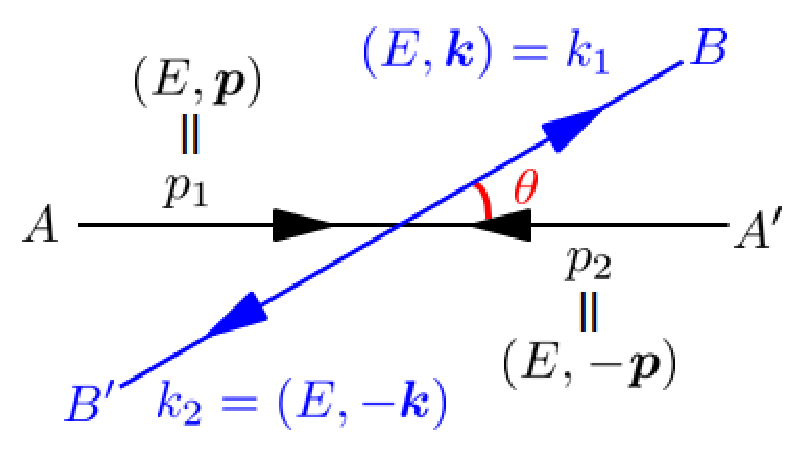
\includegraphics[width=165pt]{graphics/collision.eps}
\end{minipage}
\begin{minipage}{270pt}
\begin{align*}
 \vnorm p ^2 &= E^2-m_A^2 & \vipro pk &=\vnorm p \vnorm k\cos\theta\\
 \vnorm k ^2 &= E^2-m_B^2
\end{align*}
\begin{align*}
 p_1 \cdot p_2&=s/2-m_A^2 & p_1\cdot k_1  &= p_2 \cdot k_2 = \tfrac12(m_A^2+m_B^2-t);\\
 k_1 \cdot k_2&=s/2-m_B^2 & p_1 \cdot k_2 &= p_1 \cdot k_2 = \tfrac12(m_A^2+m_B^2-u);
\end{align*}
\end{minipage}
\begin{align*}
&&  s&= 4E^2,\\
 (p_1-p_2)^2&=-4(E^2-m_A^2)&
 t&= -(2E^2-m_A^2-m_B^2)+2\vipro pk\\
 (k_1-k_2)^2&=-4(E^2-m_B^2)&
 u&= -(2E^2-m_A^2-m_B^2)-2\vipro pk\\
\end{align*}
\paragraph{Kinematics of Collision (initial massless)}
\begin{align*}
 s&= 4E^2,&
 (t,u) &= -2E^2+\frac{m_1^2+m_2^2}{2}\pm2\vipro pk,&
 \vnorm k ^2 &= E^2-\frac{m_1^2+m_2^2}{2}+\frac{\left(m_1^2-m_2^2\right)^2}{16 E^2}
\end{align*}
\TODO{needs check}
\newpage
\subsection{楊-Mills Theory}\label{sec:yang-mills-general}
\vspace{-22pt}\hskip160pt{\small(See App.~\ref{sec:yang-mills-theory} for verbose notes.)}
\subsubsection{Non-Abelian gauge theory}
\begin{align*}
  [T^a,T^b] &= \ii f\T^a^b_c T^c,&
  &0 =f\T^D_a_b f\T^E_D_c + f\T^D_c_a f\T^E_D_b  + f\T^D_b_c f\T^E_D_a,&
  &\Dm               =  \Pm-\ii g A_\mu\\
 \Tr T^aT^b&=\frac12\delta^{ab}, &
 &[\tilde T^a]\T_i^j := T^{{\rm ad}\ a}\T_i^j :=-\ii f^{aij}&
&[\tilde\Dm]\T_i^j:=\delta_i^j\Pm+gf^{iaj}A^a_\mu.
\end{align*}
\begin{align*}
 F_{\mu\nu}        &=       \frac\ii g\left[\Dm,\Dn\right]&
 \Dm\phi                      &= \Pm\phi-\ii g A_\mu^a(T^a_\phi\phi)\\
                   &= \Pm A_\nu-\Pn A_\mu+\frac g\ii\left[A_\mu,A_\nu\right]&
 \Dm F_{\mu\nu}{}^a           &= \Pm F^a_{\mu\nu}    + g f^{abc} A_\mu^b F^c_{\mu\nu},\\
                   &=       \Bigl[\Pm A^a_\nu-\Pn A^a_\mu+gf^{abc}A_\mu^b A_\nu^c\Bigr]T^a&
 \Big(\Dm F_{\nu\rho}         &= \Pm\lambda -\ii g [A_\mu,F_{\nu\rho}]\Big).\footnotemark
\end{align*}
\footnotetext{Note that we can use any representation $T^a$ but must the same ones for $A^a_\mu T^a$ and $\lambda^a T^a$.}
\begin{align*}
 \phi              &\mapsto  V\phi := \ee^{\ii g\theta}\phi&
 A_\mu             &\mapsto  V\left(A_\mu+\frac\ii g\Pm\right)V^{-1}&
 F_{\mu\nu}        &\mapsto  VF_{\mu\nu}V^{-1}\\
 \phi^a      {}'   &\simeq \phi+\ii g \theta^aT^a\phi&
 A_\mu^a     {}'   &\simeq A_\mu^a+\Pm\theta^a+gf^{abc}A_\mu^b\theta^c&
 F_{\mu\nu}^a{}'   &\simeq F_{\mu\nu}^a+g f^{abc}F_{\mu\nu}^b\theta^c
\end{align*}
\begin{equation*}
 \epsilon^{\mu\nu\rho\sigma}\left[\Dn,\left[\Dr,\Ds\right]\right] = \epsilon^{\mu\nu\rho\sigma}\Dn F_{\rho\sigma} = 0.
\end{equation*}

\paragraph{Killing and Casimir}
Here we have two constants which {\bf depend on representation $r$}.
\begin{equation}
    \Tr(T^aT^b) =: C(r)\delta^{ab}\quad \text{\footnotesize(Killing form)},\qquad
    T^aT^a =: C_2(r)\cdot\vc 1\quad \text{\footnotesize(quadratic Casimir operator)},
\end{equation}
which satisfy
\begin{align}
   C(r) &= \frac{d(r)}{d(\text{ad})}C_2(r),&
 T^aT^bT^a&=\left[C_2(r)-\frac12 C_2(\text{ad})\right]T^b,\\
 f^{acd}f^{bcd} &= C_2(\text{ad})\delta^{ab},&
 f^{abc}T^bT^c &= \frac\ii2 C_2(\text{ad})T^a.
\end{align}


\subparagraph{For $\gSU(N)$}For its fundamental representation $N$ with definition $C(N):=\frac12$, we have
\begin{align*}
  C(N)&:=\frac12, & C_2(N)&= \frac{N^2-1}{2N}, & C(\text{ad}) =
 C_2(\text{ad}) &= N;&
  (T^a)_{ij}(T^a)_{kl} &= \frac12\left(\delta_{il}\delta_{kj}-\frac{\delta_{ij}\delta_{kl}}{N}\right).
\end{align*}

\subsubsection{Abelian gauge theory}\label{sec:abelian-gauge-theory}
In Abelian gauge theory, $V$ and fields are always commutative, and thus we have charge freedom ($Q$).
\begin{align*}
 \Dm\phi           &=       \left(\Pm-\ii g A_\mu Q\right)\phi&
 &\phi              \mapsto  \ee^{igQ\theta}\phi&
 &F_{\mu\nu}        =       \frac\ii g\left[\Dm,\Dn\right] = \Pm A_\nu-\Pn A_\mu\\
 \Dm\lambda^a     &=       \Pm\lambda^a&
 &A_\mu             \mapsto  A_\mu + \Pm\theta&
 &F_{\mu\nu}        \mapsto  F_{\mu\nu}
\end{align*}

\subsubsection{Lagrangian Block}
\begin{align}
 &\Lag \ni \left|\Dm\phi\right|^2-m^2|\phi|^2, \quad
          \overline\psi(\ii\slashed\DD-m)\psi,\quad
          -\frac14F_a^{\mu\nu}F^a_{\mu\nu}\ \Bigl(=-\frac12\Tr F^{\mu\nu}F_{\mu\nu}\Bigr),\quad
          \theta\epsilon^{\mu\nu\rho\sigma}F^a_{\mu\nu}F^a_{\rho\sigma}\\
 &-\frac14F_a^{\mu\nu}F^a_{\mu\nu}
  = -\frac12\left[
       (\Pm A^a_\nu)^2 +A^a_\mu\Pmu\Pnu A^a_\nu
 \right]
    - gf^{abc}A_\mu^a A_\nu^b \Pmu A^{c\nu}
    - \frac{g^2}4 f^{abc}f^{ade}A^b_\mu A^c_\nu A^{d\mu}A^{e\nu}
\end{align}

\subsection{$\gSU(2)$ Gauge Group}
The $\gSU(2)$ is defined as $[T^a,T^b]=\ii\epsilon^{abc}T^c$.
The representation whose generator is $\tau^a:=\sigma^2/2$ is called the fundamental representation $\boldsymbol 2$.
\subsubsection{Gauge singlet of $\gSU(2)$}
Consider the fields which transform under $\boldsymbol2$,
\begin{equation}
 \phi\mapsto \phi+\ii g\theta^a\left(\tau^a\phi\right).
\end{equation}
For scalar fields $\phi$ and vector fields $v$, it is obvious that $\phi^\dagger\phi' (=\phi^*_a \phi'_a)$ and $v^\mu v'^*_\nu$ are gauge singlet.

Fermions are Lorentz symmetric under the form
 $\xi^\alpha\chi_\alpha$.
So, in order to make a gauge and Lorentz invariant term, we have to build $\overline{\boldsymbol 2}$ representation. It can be done with $\sigma^2$:
\begin{equation}\begin{split}
  \delta(\sigma^2\xi^\alpha) &=
\sigma^2\cdot\ii g\theta^a\left(\tau^a\xi^\alpha\right)
=
\ii g\theta^a\left(\sigma^2\tau^a\sigma^2\right)\left(\sigma^2\xi^\alpha\right)
=
-\ii g\theta^a\trans{\tau^a}\left(\sigma^2\xi^\alpha\right)
,\\
& \text{i.e.,}\quad \trans{(\xi^\alpha_a\sigma^2)}\mapsto\trans{(\xi^\alpha\sigma^2)}-\ii g\theta^a\cdot\trans{(\xi^\alpha\sigma^2)}\tau^a
\end{split}\end{equation}
Thus $\sigma^2\xi^\alpha$ follows $\overline{\boldsymbol 2}$ representation, and
$(\sigma^2\xi^\alpha)\chi_\alpha=\ii\epsilon_{ab}(\xi_a)^\alpha(\chi_b)_\alpha$ is invariant under gauge and Lorentz transformation.


In summary, Weyl (Dirac) spinors $\xi$ ($\psi$) in ${\boldsymbol 2}$ representation composes a gauge singlet in the form of
\begin{equation}
 \epsilon_{ab}\xi_a\xi'_b \qquad (\overline\psi \psi').
\end{equation}

\subsubsection{$\boldsymbol 3$ representation}
Let us consider a field $\phi$ whose $\gSU(2)$ charge is $\boldsymbol 3$:\footnote{
Note that the representation $\left\{
\dfrac1{\sqrt2}\pmat{0&1&0\\1&0&1\\0&1&0},
\dfrac\ii{\sqrt2}\pmat{0&-1&0\\1&0&-1\\0&1&0},
\pmat{1&0&0\\0&0&0\\0&0&-1}
\right\}$ is equivalent to $J^A$.}
\begin{equation}
 \phi\mapsto\exp\left(\ii g\theta^A J^A\right)\phi
\qquad\text{with}\quad [J^A]_{bc}=-\ii\epsilon^{Abc}.
\end{equation}
Then,
\begin{equation}
 \phi^a\tau^a\mapsto
\ee^{\ii g\theta^A\tau^a}
 \left(\phi^a\tau^a\right)
\ee^{-\ii g\theta^A\tau^a}.
\end{equation}
It is convenient to define $\sigma^\pm$ and  $\phi^\pm$ as
\begin{align}
 \phi^\pm   &:= \frac1{\sqrt2}(\phi^1\mp\ii\phi^2),&
 \sigma^+ &:= \pmat{0&1\\0&0},&
 \sigma^- &:= \pmat{0&0\\1&0};&
 \phi^1          &= \frac{\phi^++\phi^-}{\sqrt2}&
 \phi^2          &= \frac{\ii(\phi^+-\phi^-)}{\sqrt2};
\end{align}
\begin{equation}
 \phi^a\tau^a = \frac12\pmat{\phi^3&\sqrt2\phi^+\\\sqrt2\phi^-&-\phi^3}
=\frac{\sigma^+}{\sqrt2}\phi^+
+\frac{\sigma^-}{\sqrt2}\phi^-
+\frac{\sigma^3}{2}\phi^3.
\end{equation}

%%% Local Variables:
%%% TeX-master: "CheatSheet.tex"
%%% End:
